\documentclass{standalone}
\usepackage{tikz}
\usetikzlibrary{patterns, positioning}
\usepackage[sfdefault]{ClearSans} %% option 'sfdefault' activates Clear Sans as the default text font
\usepackage[T1]{fontenc}

\begin{document}
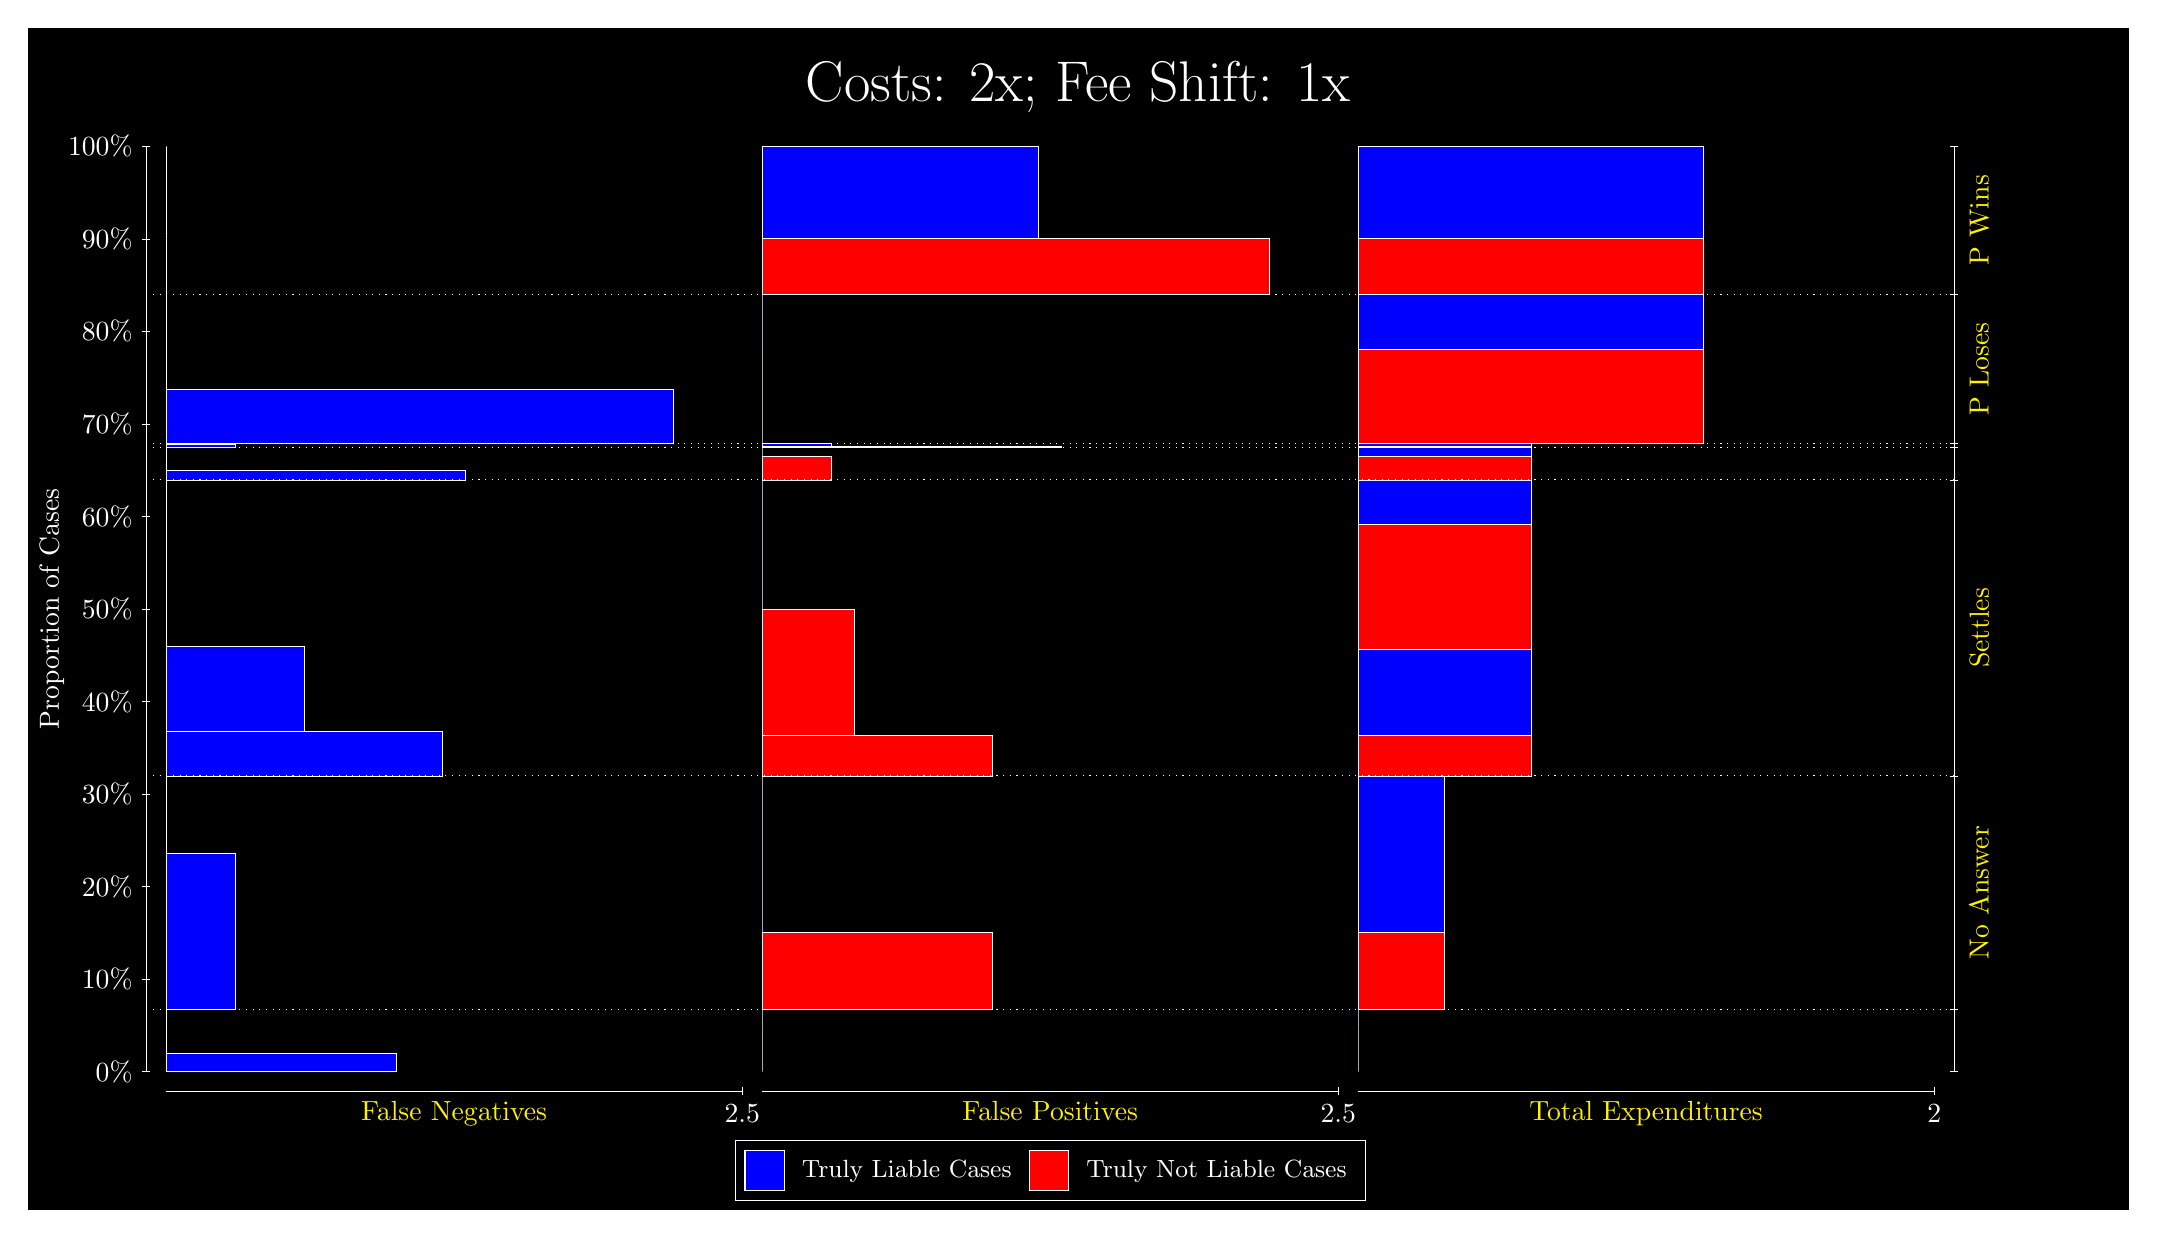
\begin{tikzpicture}
\draw[fill=black] (0,0) rectangle (26.667,15);
\draw[text=white] (0,13.5) rectangle (26.667,15) node[midway] {\huge Costs: 2x; Fee Shift: 1x};
\draw[white, very thin] (1.5,1.75) -- (1.5,13.5);
\node[rotate=90, text=white, anchor=center] at (0.3, 7.625) {Proportion of Cases};
\draw[white, very thin] (1.45,1.75) -- (1.55,1.75);
\node[text=white, anchor=east] at (1.45, 1.75) {0\%};
\draw[white, very thin] (1.45,2.925) -- (1.55,2.925);
\node[text=white, anchor=east] at (1.45, 2.925) {10\%};
\draw[white, very thin] (1.45,4.1) -- (1.55,4.1);
\node[text=white, anchor=east] at (1.45, 4.1) {20\%};
\draw[white, very thin] (1.45,5.275) -- (1.55,5.275);
\node[text=white, anchor=east] at (1.45, 5.275) {30\%};
\draw[white, very thin] (1.45,6.45) -- (1.55,6.45);
\node[text=white, anchor=east] at (1.45, 6.45) {40\%};
\draw[white, very thin] (1.45,7.625) -- (1.55,7.625);
\node[text=white, anchor=east] at (1.45, 7.625) {50\%};
\draw[white, very thin] (1.45,8.8) -- (1.55,8.8);
\node[text=white, anchor=east] at (1.45, 8.8) {60\%};
\draw[white, very thin] (1.45,9.975) -- (1.55,9.975);
\node[text=white, anchor=east] at (1.45, 9.975) {70\%};
\draw[white, very thin] (1.45,11.15) -- (1.55,11.15);
\node[text=white, anchor=east] at (1.45, 11.15) {80\%};
\draw[white, very thin] (1.45,12.325) -- (1.55,12.325);
\node[text=white, anchor=east] at (1.45, 12.325) {90\%};
\draw[white, very thin] (1.45,13.5) -- (1.55,13.5);
\node[text=white, anchor=east] at (1.45, 13.5) {100\%};

\draw[white, very thin] (24.457,1.75) -- (24.457,13.5);
\draw[white, very thin] (24.407,1.75) -- (24.507,1.75);
\node[anchor=west] at (24.407, 1.75) {};
\draw[white, very thin] (24.407,2.5386) -- (24.507,2.5386);
\node[anchor=west] at (24.407, 2.5386) {};
\draw[white, very thin] (24.407,5.5046) -- (24.507,5.5046);
\node[anchor=west] at (24.407, 5.5046) {};
\draw[white, very thin] (24.407,9.2639) -- (24.507,9.2639);
\node[anchor=west] at (24.407, 9.2639) {};
\draw[white, very thin] (24.407,9.6796) -- (24.507,9.6796);
\node[anchor=west] at (24.407, 9.6796) {};
\draw[white, very thin] (24.407,9.7239) -- (24.507,9.7239);
\node[anchor=west] at (24.407, 9.7239) {};
\draw[white, very thin] (24.407,11.623) -- (24.507,11.623);
\node[anchor=west] at (24.407, 11.623) {};
\draw[white, very thin] (24.407,13.5) -- (24.507,13.5);
\node[anchor=west] at (24.407, 13.5) {};

\draw[white, very thin, fill=blue] (1.75,1.75) rectangle (4.6775,1.9772);
\draw[white, very thin, fill=red] (1.75,1.9772) rectangle (1.75,2.5386);
\draw[white, very thin, fill=blue] (1.75,2.5386) rectangle (2.6283,4.5253);
\draw[white, very thin, fill=red] (1.75,4.5253) rectangle (1.75,5.5046);
\draw[white, very thin, fill=blue] (1.75,5.5046) rectangle (5.2631,6.066);
\draw[white, very thin, fill=blue] (1.75,6.066) rectangle (3.5065,7.1523);
\draw[white, very thin, fill=red] (1.75,7.1523) rectangle (1.75,9.2639);
\draw[white, very thin, fill=blue] (1.75,9.2639) rectangle (5.5558,9.3798);
\draw[white, very thin, fill=red] (1.75,9.3798) rectangle (1.75,9.6796);
\draw[white, very thin, fill=blue] (1.75,9.6796) rectangle (2.6283,9.7109);
\draw[white, very thin, fill=red] (1.75,9.7109) rectangle (1.75,9.7239);
\draw[white, very thin, fill=blue] (1.75,9.7239) rectangle (8.1906,10.419);
\draw[white, very thin, fill=red] (1.75,10.419) rectangle (1.75,11.623);
\draw[white, very thin, fill=red] (1.75,11.623) rectangle (1.75,12.329);
\draw[white, very thin, fill=blue] (1.75,12.329) rectangle (1.75,13.5);
\draw[white, very thin, fill=red] (9.3189,1.75) rectangle (9.3189,2.3114);
\draw[white, very thin, fill=blue] (9.3189,2.3114) rectangle (9.3189,2.5386);
\draw[white, very thin, fill=red] (9.3189,2.5386) rectangle (12.246,3.518);
\draw[white, very thin, fill=blue] (9.3189,3.518) rectangle (9.3189,5.5046);
\draw[white, very thin, fill=red] (9.3189,5.5046) rectangle (12.246,6.0241);
\draw[white, very thin, fill=red] (9.3189,6.0241) rectangle (10.49,7.6162);
\draw[white, very thin, fill=blue] (9.3189,7.6162) rectangle (9.3189,9.2639);
\draw[white, very thin, fill=red] (9.3189,9.2639) rectangle (10.197,9.5637);
\draw[white, very thin, fill=blue] (9.3189,9.5637) rectangle (9.3189,9.6796);
\draw[white, very thin, fill=red] (9.3189,9.6796) rectangle (13.125,9.6926);
\draw[white, very thin, fill=blue] (9.3189,9.6926) rectangle (10.197,9.7239);
\draw[white, very thin, fill=red] (9.3189,9.7239) rectangle (9.3189,10.928);
\draw[white, very thin, fill=blue] (9.3189,10.928) rectangle (9.3189,11.623);
\draw[white, very thin, fill=red] (9.3189,11.623) rectangle (15.759,12.329);
\draw[white, very thin, fill=blue] (9.3189,12.329) rectangle (12.832,13.5);
\draw[white, very thin, fill=red] (16.888,1.75) rectangle (16.888,2.3114);
\draw[white, very thin, fill=blue] (16.888,2.3114) rectangle (16.888,2.5386);
\draw[white, very thin, fill=red] (16.888,2.5386) rectangle (17.986,3.518);
\draw[white, very thin, fill=blue] (16.888,3.518) rectangle (17.986,5.5046);
\draw[white, very thin, fill=red] (16.888,5.5046) rectangle (19.083,6.0241);
\draw[white, very thin, fill=blue] (16.888,6.0241) rectangle (19.083,7.1103);
\draw[white, very thin, fill=red] (16.888,7.1103) rectangle (19.083,8.7025);
\draw[white, very thin, fill=blue] (16.888,8.7025) rectangle (19.083,9.2639);
\draw[white, very thin, fill=red] (16.888,9.2639) rectangle (19.083,9.5637);
\draw[white, very thin, fill=blue] (16.888,9.5637) rectangle (19.083,9.6796);
\draw[white, very thin, fill=red] (16.888,9.6796) rectangle (19.083,9.6926);
\draw[white, very thin, fill=blue] (16.888,9.6926) rectangle (19.083,9.7239);
\draw[white, very thin, fill=red] (16.888,9.7239) rectangle (21.279,10.928);
\draw[white, very thin, fill=blue] (16.888,10.928) rectangle (21.279,11.623);
\draw[white, very thin, fill=red] (16.888,11.623) rectangle (21.279,12.329);
\draw[white, very thin, fill=blue] (16.888,12.329) rectangle (21.279,13.5);
\draw[white, dotted] (1.5,2.5386) -- (24.457,2.5386);
\draw[white, dotted] (1.5,5.5046) -- (24.457,5.5046);
\draw[white, dotted] (1.5,9.2639) -- (24.457,9.2639);
\draw[white, dotted] (1.5,9.6796) -- (24.457,9.6796);
\draw[white, dotted] (1.5,9.7239) -- (24.457,9.7239);
\draw[white, dotted] (1.5,11.623) -- (24.457,11.623);
\draw[white, very thin] (1.75,1.5) -- (9.0689,1.5);
\node[text=yellow, anchor=north] at (5.4094, 1.5) {False Negatives};
\draw[white, very thin] (9.0689,1.45) -- (9.0689,1.55);
\node[text=white, anchor=north] at (9.0689, 1.45) {2.5};

\draw[white, very thin] (9.3189,1.5) -- (16.638,1.5);
\node[text=yellow, anchor=north] at (12.978, 1.5) {False Positives};
\draw[white, very thin] (16.638,1.45) -- (16.638,1.55);
\node[text=white, anchor=north] at (16.638, 1.45) {2.5};

\draw[white, very thin] (16.888,1.5) -- (24.207,1.5);
\node[text=yellow, anchor=north] at (20.547, 1.5) {Total Expenditures};
\draw[white, very thin] (24.207,1.45) -- (24.207,1.55);
\node[text=white, anchor=north] at (24.207, 1.45) {2};


\node[text=yellow, centered, rotate=90] at (24.777, 4.0216) {No Answer};
\node[text=yellow, centered, rotate=90] at (24.777, 7.3842) {Settles};


\node[text=yellow, centered, rotate=90] at (24.777, 10.673) {P Loses};
\node[text=yellow, centered, rotate=90] at (24.777, 12.561) {P Wins};

\draw (12.978300999999998,1.5) node[draw=none] (baseCoordinate) {};
\begin{scope}[align=center]
        \matrix[scale=0.5, draw=white, below=0.5cm of baseCoordinate, nodes={draw}, column sep=0.1cm]{
            \node[rectangle, draw, minimum width=0.5cm, minimum height=0.5cm, fill=blue] {}; &
            \node[draw=none, font=\small, text=white] (B) {Truly Liable Cases}; &
            \node[rectangle, draw, minimum width=0.5cm, minimum height=0.5cm, fill=red] {}; &
            \node[draw=none, font=\small, text=white] (B) {Truly Not Liable Cases}; \\
            };
\end{scope}

\end{tikzpicture}
\end{document}